\newcommand{\st}{ \ | \ }

\section{Requirements for New Graph Syntax}
  \label{s:requirements}
  The goal of the new graph--based syntax presented here is to enable the general structure of an MDAO problem to be described independently of any solution information, 
  while still being able to accomodate the more specific case when a solution 
  strategy is applied. In order to achieve this goal, 
  the graph syntax needs to accomodate a number of MDAO problem constructs: 
  \begin{itemize}
    \item Analysis tools and their interconnections
    \item Design variables, objectives, and constraints
    \item Local and global information
    \item Coupling between analyses
    \item Multi-fidelity analyses
  \end{itemize}

The new syntax is intended to represent three phases of the design problem formulation process. 
In the initial problem definition
  phase, the specific analysis tools and design goals are identified. Next, 
  a single formal problem formulation is identified that specifies design variables, constraints, objectives, 
  analysis tools, and all other elements required to represent the overall MDAO problem. 
Lastly, a specific procedure for solving the problem is selected, e.g. selecting an MDAO optimization architecture. Using the proposed graph syntax, these phases 
  can be represented with the following three graphs:
  \begin{itemize}
    \item Maximal Connectivity Graph (MCG)
    \item Fundamental Problem Graph (FPG)
    \item Problem Solution Graph (PSG)
  \end{itemize}

  The \emph{maximal connectivity graph} represents the first phase of the problem formulation with all 
  analysis codes being considered and all possible connections between them also present. The second graph 
  is the \emph{fundamental problem graph}, which is the smallest possible graph 
  that still fully defines a given problem formulation that could in principle be solved by an MDAO technique. Finally, a \emph{specific problem formulation} 
  may be represented by including additional edges and nodes to represent the 
  solution strategy being employed to solve the problem. 

  The relationship between these three graphs is depicted in Figs.~\ref{f:tree} and \ref{f:hourglass}. 
  The tree diagram demonstrates the fact that it is generally possible to obtain 
  multiple FPGs from a single maximal connectivity graph. This  may correspond to 
  different down--selections of analysis codes, different connections between them, 
  or both. Each down--selection shrinks the number of possible FPGs that could be reached 
  until only one is remaining. Then, from a single FPG, different PSGs may be obtained by implementing 
  different solution strategies. If you consider the size of a graph to be the sum of all of its
  edges and nodes then the hourglass shape in Fig. \ref{f:hourglass} illustrates how
the FPG is obtained from the MCG by removing nodes and edges, 
  and the PSG is obtained from the FPG by adding nodes and edges.

  \begin{figure}[htb!]
    \centering
    \subfigure[number of possible graphs]{
    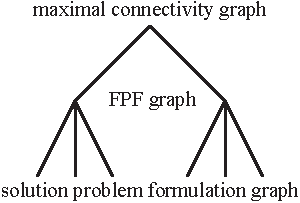
\includegraphics[width=2.0in]{images/tree}
    \label{f:tree}
    }
    \subfigure[graph size]{
    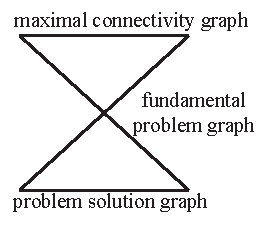
\includegraphics[width=2.0in]{images/hourglass}
    \label{f:hourglass}
    }
  \caption{The relationship between the MCG, FPG, and PSG.}
  \end{figure}

\section{Syntax Definition}
  \label{s:syntax definition}
  In this section, we present the necessary graph theoretic fundamentals to 
  construct the graphs discussed in Sec.~\ref{s:requirements}. 
  The notation used in this work is adapted from Diestel \cite{Diestel2010}. 
  A \emph{graph} is a pair $G = (V,E)$ of sets such that $E \subseteq V \times V$, 
  which means that the elements of $E$ are 2--element subsets of $V$. The set $V$ 
  contains the \emph{vertices} or \emph{nodes} and the set $E$ contains the \emph{edges}.
  For a \emph{directed graph} (or \emph{digraph}) we construct $E$ as a set of ordered pairs instead 
  of a set of sets. Each ordered pair represents an edge starting at the node 
  indicated by the first entry and directed to the node indicated by the second 
  entry. Edge $e$ = $(x,y)$ may be referred to simply as $xy$. For node $v \in V$ 
  the edges directed out from $v$ are denoted by $E(v)$ and the edges directed into $v$ are given 
  by $E^{-1}(v)$. 
  If $E$ is not a one--to--one mapping, $E(v)$ may be the empty set, a single node, or a set of nodes.
  \begin{figure}[htb!]
    \begin{center}
    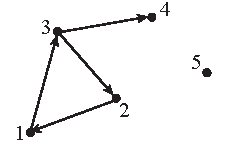
\includegraphics[width=1.5in]{images/example_directed_graph}
    \end{center}
    \vspace{-20pt}
  \caption{Example directed graph.}
  \label{f:example directed graph}
  \end{figure}
  As an example, for the directed graph shown in Fig.~\ref{f:example directed graph} we have
  \begin{IEEEeqnarray*}{rCl}
  V & = & \{1,2,3,4,5\}, \\
  E & = & \big\{(2,1),(3,2),(1,3),(3,4)\big\}.
  \end{IEEEeqnarray*}

  A \emph{path} $P=(V,E)$ from $x_0$ to $x_k$ in graph $G$ is a subgraph of $G$ with $V = \{x_0,x_1,\ldots,x_k\}$ and $E = \{(x_0,x_1),(x_1,x_2),\ldots,(x_{k-1},x_k)\}$.
  A \emph{reverse path} $P_R$ in graph $G$ is a path on $R$, where $R$ is the reverse graph of $G$ obtained by switching the orientation of every edge.


  %does this belong in the analysis block section???? 
  Let $I$ be a nonempty set such that for each $i \in I$ there is a corresponding set $A_i$. 
  The set of sets $\mathcal A = \{A_i \st i \in I\}$ is called an indexed family of sets with index $i$ and 
  indexing set $I$\cite{smith2006}. 
  The union over this family of sets can be described in a few different ways:
  \begin{equation}
  \bigcup_{i \in I} A_i = \bigcup_{A \in \mathcal A} A = \{x \st x \in A \txt{ for some } A \in \mathcal A\}.
  \end{equation}

  Lastly, the cardinality of a set $B$ is the number of elements in $B$ and is denoted as $|B|$.

\subsection{Node and Edge Types}
  \label{ss:types}
  We now define different types of nodes and edges with specific properties to compose graphs used to represent an MDAO problem. 
  There are three node types:  
  \begin{description}
    \item[variable:] represents scalar or array data
    \item[model:] responsible for mapping inputs to outputs
    \item[driver:] control logic capable of managing iteration
  \end{description}

  In addition to the three node types, there are two edge types: 

  \begin{description}
  \item[connection edge:] Exchange of information between two nodes. These edges 
  can either be fixed (cannot be removed from graph) or free (can be removed). 
  \item [driven edge:] Passing of information from a driver node to a 
    variable node. A single variable node can have many incomming driven edges. These edges are 
    free and can be added or removed from the graph. 
  \end{description}

  [[Insert legend for node and edge types]]

  In Alexandrov and Lewis's REMS syntax only two node types (variable and function) and one edge type are included \cite{alexandrov2004}. 
 We have chosen to adopt the terminology ``model'' node instead of ``function'' node to be consistent with modern MDAO framework terminonlogy. The present work 
  adds one additional node types and one additional edge type to the syntax to allow descriptive
  graphs for all three phases of the design problem formulation process. In addition, we introduce the 
  concept of fixed vs. free connection edges to represent the
  static relationship between variable and model nodes from a single analysis, 
  vs the flexible relationship between variables from different analyses. 

\subsection{Rules for Nodes and Edges}
  \label{ss:rules}
  A rule set is provided for the usage of these nodes and edges.
  The driver node and the driven edge are allowed to be present only in PSGs.
  Other node and edge types can be present in any of the three graph types, subject to the following restrictions: 
  \begin{enumerate}
  \item A model node may have only one edge directed to or from another model node.
  \item A model node may have only fixed connection edges directed in or out.
  \item A model node must have at least one edge directed in and at least one edge 
    directed out.
  \item If a variable node has an outgoing edge to a model node, then it may not have other outgoing edges.
  \end{enumerate}

\subsection{indegree and outdegree}
  \label{s:indegree-outdegree}
  The \emph{indegree} of a node is the number of connection edges directed in and 
  is denoted as $\txt{deg}^-(v)$, and the \emph{outdegree} 
  is the number of connection edges directed out and it is denoted as $\txt{deg}^+(v)$.
  The degree of a given node is a function only of the connection edges 
  attached to it. The number of driven edges is not relevant because any number 
  of drivers could be involved in different parts of an solution process. For 
  example in a sequential optimization in which a global optimizer is used first 
  followed by a gadient based optimizer second to refine global optimizer 
  result, design variables would have incomming driven edges from both optimizers. 
  These driven edges would not affect the indegree of those variable nodes. 

  Specifially for variable nodes we also define the \emph{upper indegree limit} 

  \begin{equation}
  \txt{deg}_u^-(v):V \to \mathbb{N}
  \end{equation} 
  and the \emph{lower indegree limit} as
  \begin{equation}
  \txt{deg}_l^-(v):V \to \mathbb{N}.
  \end{equation}
  These user-specified limits govern the number of connection edges that may 
  be directed into a variable node for a valid graph. Consider a variable 
  node $v$ with $\txt{deg}_u^-(v) = \txt{deg}_l^-(v) = 1$. In this case, $v$ 
  must have exactly one incomming explicit edge or the graph is deemed invalid. 
  Two possiblities exist for voilating these limit conditions: 

  \begin{description}
    \item[hole: ] The number of incomming edges is less than the lower indegree limit:
      \begin{equation} \txt{deg}^-(v) < \txt{deg}_l^-(v) \label{e:hole} \end{equation}
      A hole represents a lack of information being supplied to the node.
    \item[collision: ] The number of incomming edges is greater than $ \txt{deg}_u^-(v)$. 
      \begin{equation} \txt{deg}^-(v) > \txt{deg}_u^-(v) \label{e:collision}\end{equation}
  \end{description} 

  The presence of holes and collisions in a graph represent issues that will give
  rise to an invalid problem formulation. An algorithm for detecting and 
  managing these violations if proposed in Sec.~\ref{s:building graphs}.\ref{ss:obtaining FPG}.

\section{Graph Representation of MDAO Constructs}
\label{s:graph representation}
In this section we present our graph syntax applied to the description of MDAO 
Problems. We make use of the Sellar problem, described in 
Eq. \ref{eqn:simple_fpf} as an example to illustrate the implementation of the syntax. 
The graph representation of the Sellar problem, using the new stynax, is 
presented in Fig. \ref{f:sellar_graph_full}. In this section sub-graphs or 
slight modifications of the full graph will be used to demonstrate the 
important MDAO constructs described by this graph syntax.

\begin{figure}[htb!]
    \begin{center}
    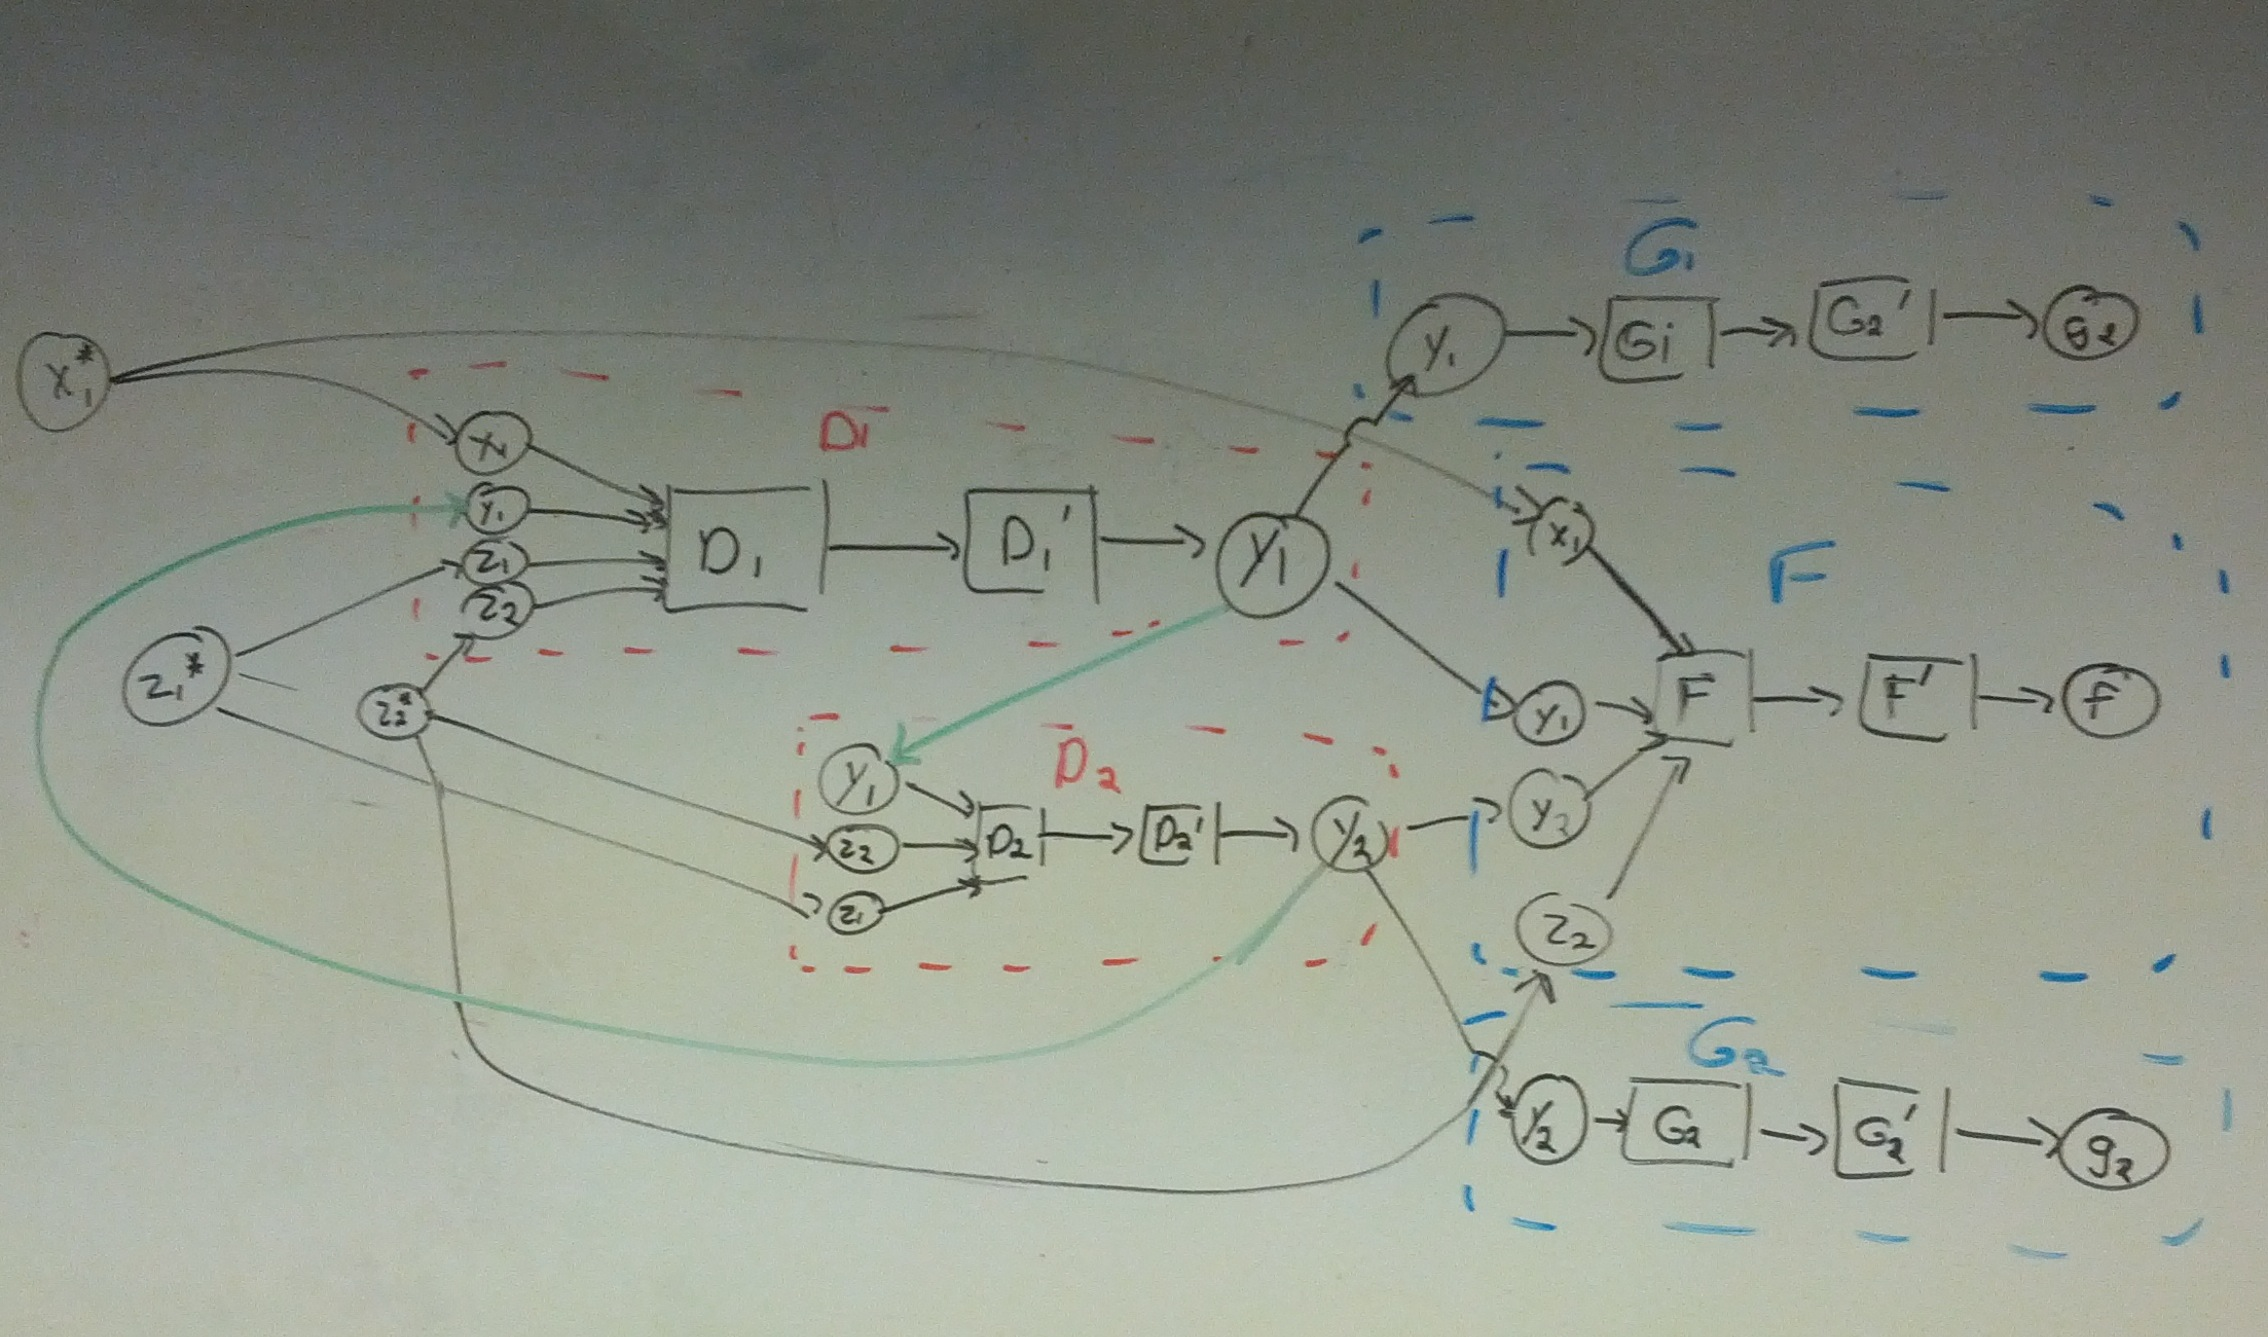
\includegraphics[width=4in]{images/sellar_graph_full}
    \end{center}
    \vspace{-10pt}
\caption{Graph of the Sellar problem formulation}
\label{f:sellar_graph_full}
\end{figure}

\subsection{Analysis Blocks and Connections}
\label{ss:analysis blocks and connections}
Analysis tools take in a number input variables and then calculate 
the values for their respective outputs. We represent this process
by a group of nodes and edges called an \emph{analysis block}, 
shown in Fig. \ref{f:analysis block}. Within an analysis block, each variable 
node represents a single input or output and is connected 
to a single model node via a fixed edge. Note that in Fig.~\ref{f:analysis block}, 
the analysis block includes two model nodes, with a single edge connecting them. 
This edge represents the necessary calculations to map given inputs 
to the outputs of the anlysis. This calculation edge provides the opportunity 
to encode computational cost or other characteristics of the analysis code as 
a weight in a weighted graph formulation. If associating a weight is 
unnecessary, the calculation edge may be omitted and all input and output 
variables can be connected to a single model node for a given analysis block. 
Since all the edges within analysis blocks are fixed, the blocks themselves are 
fixed sub-graphs within the overall MDAO problem graph. The connectivity of 
nodes and edges in an analysis block cannot be altered for the purposes of MDAO 
problem formulation; however, analysis block sub-graphs can be added or removed 
from the MDAO problem graph as needed.

\begin{figure}[htb!]
    \begin{center}
    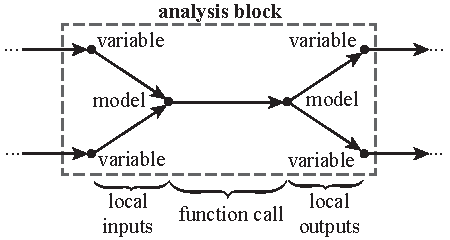
\includegraphics[width=4in]{images/analysis_block}
    \end{center}
    \vspace{-10pt}
\caption{Example analysis block. The each node type and edge type is labeled in italics and annotated parenthetically.}
\label{f:analysis block}
\end{figure}

Variable nodes in an analysis block can be distinguished as either an input or 
an output by the manner in which they are connected. As shown in Fig.~\ref{f:analysis block}, 
inputs are represented as variable nodes that have an outgoing edge into a model 
node. Conversely, outputs represented as any variable nodes that have an incoming 
edge from a model node. 

MDAO problems require that information be passed between sets of analyses. When 
information from one output of an analysis block is passed, or connected, to an 
input of another analysis block, a new connection edge is added between the two 
variable nodes involved in the exchange. These connection edges are free, and unlike the edges 
within an analysis block, the edges can be added or removed depending on the needs
of a given design problem. In other words, free connection edges are created by 
engineers linking an output of one tool to an input of another one. It is 
allowable for a single output to have outgoing connection edges to multiple 
downstream inputs. 

\subsection{Design Variables}
Design variables are the input variables that are free to be 
changed by the designer or by an optimizer in an MDAO study. In a graph design
variables will be a set of variable nodes, $V_{dv}$, identified as follows: 

\begin{equation}
  V_{dv} = \{V \st \txt{deg}_l^-(v)=0\}
\end{equation}

For the Sellar problem, there are three design variables: $x_1^*$, $z_1^*$, and 
$z_2^*$. In Fig. \ref{f:designvars} all variable from the Sellar problem are 
annotated with their lower indegree limit and the three design variables are identified 
in bold. 

\begin{figure}[htb!]
  \begin{center}
    [Graph Here....]
    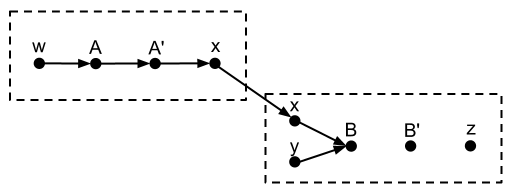
\includegraphics[width=.6\textwidth]{images/design_vars_graph}
  \end{center}
  \caption{Sellar problem graph with lower indegree limits for all variables \label{f:designvars}}
\end{figure}

In Fig. \ref{f:designvars}, none of the design variable nodes have any incomming 
edges. In general, in a MCG or a FPG, design variables will 
show up as nodes without any incomming edges. For a valid PSG, design variables 
could have one or more incomming driven edges representing a value determined by 
a optimizer. 

Note the although there are no incomming edges, design variables are not holes 
in the graph as defined by Eq. \ref{e:hole}. Since they have $\txt{deg}_l^-(v)=0$ 
having no incomming connection edges does not violate their lower indegree limit. 
However, the concept of holes can be useful for identifying potential design variables
given an arbitrary MCG. If you first set $\txt{deg}_l^-(v)=1$ for all variable nodes, 
and then find the resulint holes, you will have a list of variable nodes that 
could potentially be design variables. Some variables will be true design variables, 
while others might represent missing information in the problem formulation. For 
instance, if there is a hole for a drag input of an aircraft mission analysis code 
then this is not likely a good choice for a design variable. So it is up to the designer to 
examine each hole and decide if it's an appropriate design variable. If 
the variable should become a design variable then set $\txt{deg}_l^-(v)=0$. 
If a variable should not be a design variable, then leave it as a hole which 
needs to be addressed in a manner discussed in section \ref{ss:obtaining FPG}.
 

\subsection{Objectives and Constraints}
\label{ss:objectives and constraints}
Objectives and constraints are constructs that need to be identified when 
describing and MDAO problem. In the case of objective functions a single output 
value generated by an analysis block could be selected, but commonly multiple 
values are assembeled together to form a composite objective function. 
Generally both objective and constraint functions accept a set of inputs and map 
them to an output value of significance to the overall design problem. 

The operations of implementing composite objective and constraint functions, 
although typically simple, are effectively the identical to the task performed by an 
analysis block. A composit constraint or objective function can therfore 
be represented as an additional analysis block within the graph, with its own input and 
output variable nodes. Although fundamentally no different than an analysis block, 
for clarity and convience, it is useful to distinguish between analysis 
blocks corresponding to analysis codes and those that arise from the addition of 
objectives or constraints to the graph. Therefore, we define an 
\emph{expression block}, as the collection of variable and model nodes related 
to a given objective or constraint function. Fig. \ref{f:obj-cons} highlights 
the objective and constraint blocks from the Sellar problem. If the relevant 
objective and constraint values are direct results from other analysis blocks 
and composite functions are not needed, then expression blocks may be omitted 
from the MDAO problem graph.

\begin{figure}[htb!]
  \begin{center}
    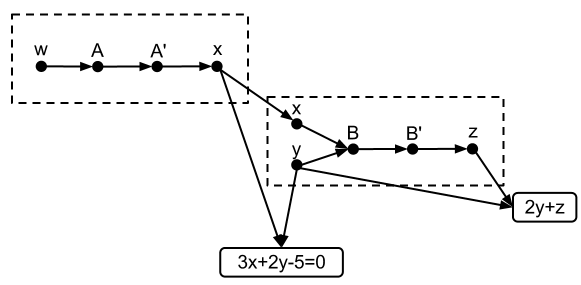
\includegraphics[width=.6\textwidth]{images/obj_const_graph}
  \end{center}
  \caption{Notional graph with and objective and constraint nodes \label{f:obj-cons}}
\end{figure}

\subsection{Local vs Global Nodes}

  The set of local nodes, $V_l$, is the collection of 
  nodes with exactly one outgoing connection edge. 

  \begin{equation}
    V_{l} = \{V \st \txt{deg}^+(v)=1\}
    \label{e:local_definition}
  \end{equation}

  In section \ref{s:specific vs fundamental} variable nodes that are part of 
  an analysis block are inherently local and similarly model nodes 
  are also local. Following the definition in Eq. \ref{e:local_definition}
  we can now see why. Variable nodes connected to model nodes are only allowed to 
  have one outgoing edge, and hence will always by definition be local variables. 

  The set of global nodes, $V_g$, is the collection of all nodes with more than 
  one outgoing connection edge. 

  \begin{equation}
    V_{g} = \{V \st \txt{deg}^+(v)>1\}
    \label{e:global_definition}
  \end{equation}

  Follwoing our definition any variable node that had multiple 
  outgoing edges, is global. In Fig. \ref{f:sellar_graph_full} 
  the variable nodes for $x_1^*$, $z_1^*$, and $z_2^*$ have multiple outgoing 
  edges and would be considered global. 

  The variable $x_1$ from the Sellar problem is usually refered to as 
  a local variable, which is contradicted by the given graph. This discrepancy 
  arises from the explicit treatment of objectives and constraints as separate 
  expression blocks. Normally in the Sellar problem, $x_1$ is considered a local 
  variable because it directly affects only analysis block $D_1$. By expanding
  $F$ into an expression block with its own inputs, then $F$ is assigned its own local 
  copy of the $x_1$ variable. This formulation necessitates the creation of the global $x_1^*$ 
  node in the graph with two outgoing edges to link the two $x_1$ inputs nodes 
  in the different blocks. Interestingly, the classification of $x_1^*$ 
  as a global variable fits nicely within the structure of the Colaborative 
  Optimization (CO) archtiecture \cite{braun1996thesis}. The rules for setting up 
  a problem with CO require that each discipline be given an independent local 
  copy of all global variables. All local variables are retained uniquely 
  within their respective disciplines, except when a local design variable appears 
  explicitely in the objective or global constraint. In that case a global 
  variable is created, and the analysis block again is again assigned an 
  independent local copy of it. Given our definition of global vs local variable 
  nodes, no such exception for local variables in global expressions is 
  necessary. Whenever a given variable is included in an expression block, 
  it forces the creation of a global variable node in the graph which will 
  result in the correct structure for CO automatically. 

  Analysis and expression blocks can themselves be local or global, but the 
  criteria for determining this is slightly different than for variable nodes. 
  In this case, you consider the set of connection edges for the block
  (e.g. from all the variable nodes within the block) as a set. Additionally, 
  you must consider both incoming and outgoing edges, where for variables 
  only outgoing connection edges were relevant. 

  A local analysis block is 
  defined as a block with incomming edges from exactly one other analysis 
  block and outgoing edges from exactly one other analysis block. A global 
  analysis block is defined as a block with incomming edges or outgoing edges 
  to more than one analysis block. 

  [[MATH HERE]]

  Looking at the Sellar problem in 
  Fig. \ref{f:sellar_graph_full} we see the expression blocks for each constraint, 
  $G_1$ and $G_2$. Both constraints are local to their respective analysis 
  blocks. But the expression block for $F$ has incomming edges from $D_1$ and 
  $D_2$, so it would considered global. 

  Catagorizing any node or analysis block block with incomming or outgoing edges
  from more than one source as global neglects a more 
  subtle aspect of some MDAO problems. Namley the locality of any node in a graph is 
  a relative property. For instance, a single node might have outgoing edges 
  to two separate analysis blocks, $A$ and $B$, but none to a third, $C$. This 
  node was global with respect to $A$ and $B$ separately, but local 
  to the group $A,B$. This situation produces a natural hierarchy in a graph, 
  from which one could form ever smaller groups as the problem is segmented into 
  finer localities. 

  When solving a problem using a hierarchical decomposition approach, 
  there are various techniques for partitioning a problem into hierarchical 
  localities that are effective in different scenarios \cite{krishnamachari1997optimal,michelena1997hypergraph,sobieszczanski1997,Perez2004,allison2009optimal}. 
  Tosserams \textit{et al.} proposed a language based-syntax for describing the 
  partitioning of problems, named $\Psi$\cite{tosserams2010specification}. 
  $\Psi$ provides an opposing perspective to this work, where they compose 
  hierarchies from the bottom up, into larger and larger groups. However, 
  $\Psi$ provides a compiler that can produce a standard problem representation 
  of the assembled problem and a number of example converters from that 
  standard representation to application specific formats. 

\subsection{Coupling Between Analyses}

  Coupling exists in a design problem when a set of two or more analyses each depend on the
  other's outputs. In the Sellar problem from Eqn \ref{eqn:simple_fpf} the two 
  coupling constraints, $H_1$ and $H_2$, provide a reciprical dependence between 
  $D_1$ and $D_2$. In a graph, these constraints appear as connection edges between 
  the outputs of each analysis block. The relevant connection edges are highlighted in 
  Fig. \ref{f:coupling}, where they form a closed path between two analysis blocks,
  called a cycle. Cycles of connection edges are the characteristic structure that 
  represents coupling. 

  \begin{figure}
      \begin{center}
      %\includegraphics[height=.25\textheight]{}
      [INSERT GRAPH HERE]
      \caption{Graph of a notional problem with simple coupling \label{f:coupling}}
      \end{center}
  \end{figure}

  Coupling cycles do not contain driver nodes in the MCG of FPG representation. 
  Solvers, optimizers, and other iterative processes are not invovled in the coupling 
  definition--though one will be necessary to build a valid PSG from a given FPG. 
  Additionally, a coupling cycle has no inherent start or end. It would be acceptable to select
  node in the cycle as a starting point and proceed around the
  loop until you get back to the starting point. For the Sellar Problem, selecting 
  $D_1$ as the starting point would yield a problem as given in 
  Eq.~\ref{eqn:simple}, whereas selecting $D_2$ would yield the problem as given in 
  Eq.~\ref{eqn:simple2}.

  Larger problems can contain more complex cycles in their FPG, indicating more 
  complex coupling between analyses. For example A cycle can involve more than 
  just two analysis blocks. Multiple independent cycles could also exist, indicating 
  independent coupling relationships. Cycles can also overlap, meaning that the same analysis 
  blocks are involved in multiple different coupling cycles. All of these situations
  arise naturally as the size of problems grows, and managing this coupling may
  become difficult. In the present work, Sec.~\ref{s:example problem}.\ref{ss:obtaining an FPG} 
  demonstrates how building an FPG from an MCG provides an opportunity to 
  identify and potentailly reduce the number of cycles in a graph. 

  If many couplings are present, convergence rates can be improved by 
  searching for an effective ordering for the execution of analyses.
  Rogers' DEMAID tool uses a genetic algorithm to find an ordering that minimizes 
  the overall coupling of the system by separating independent cycles in the 
  graph \cite{rogers1996,rogers1996demaid}. Rogers work focused on the matrix 
  form of the DSM for ordering optimization. Lu and Martins more recently leveraged 
  a weighted form of the DSM and used an iterative clustering approach to perform a 
  similar task to DEMAID \cite{Lu2012}. 

\subsection{Multi--fidelity Problems}
  \label{ss:multi-fideliy problems}
  A multi--fidelity problem can be characterized by two or more different analyses 
  each calculating the same data. Representing this type of multi--fidelity 
  construct in a graph will yield two analysis blocks, each with its own output 
  variable nodes, having outgoing edges that connect to a single variable in a 
  third analysis block that needs the data as input. So the set of all multi-fidelity
  variables, $V_{mf}$, is given as: 

  \begin{equation}
    V_{mf} = \{ V \st \txt{deg}^-(v)>1 \} \cup \{ V \st \txt{deg}^-_u(v)>=\txt{deg}^-(v) \}
  \end{equation}

  In a multi-fidelity problem, a given variable node may have multiple incomming 
  edges without causing a collision as defined by by Eq.~\ref{e:collision}. 
  Fig.~\ref{f:collision_example} shows a modified version of the Sellar problem 
  with a new analysis, $D_0$, representing a low fidelity version of $D_1$. 
  In this modified graph, the annotations indicate the upper indegree limit. For 
  $D_2$, $\txt{deg}^-_u(D_2.y_1) = 2$ which avoids a collsion. A  
  $\txt{deg}^-_u(v) > 1$ for any variable in a graph represents a decision to 
  allow multiple fidelities to interact at that part of the graph in order to alieviate
  a conflict. In section \ref{ss:obtaining FPG} we present an algorithm for finding 
  conflicts within a given MCG so that a designer can make the necessary decisisons about each 
  one in turn. 

  \begin{figure}
    \begin{center}
      %\includegraphics[height=.25\textheight]{}
    [INSERT GRAPH HERE]
    \caption{Graph of the modified Sellar, multi--fidelity problem with $\txt{deg}^-_u(v)$ annotations on variable nodes\label{f:collision_example}}
  \end{center}
  \end{figure}

  Multi--fidelity problems are always charaterized by graphs with variable 
  nodes that have an $\txt{deg}^-_u(v) > 1$. These problems require 
  special techniques for resolving the confliciting edges by introducing some mechanism
  to manage when each of the different fidelity analyses are 
  run\cite{march2012provably,alexandrov2001approximation,Huang_Allen_Notz_Miller_2006}.
  The specifics of this mechanism are not given in any form withing an MCG or 
  FPG. Instead the multi-fidelity mechanism specifics would be represented as a 
  driver in a PSG derived from any given multi-fidelity FPG. 


